\documentclass[12pt, a4paper]{article}

% Idioma y codificación (compatible con pdfLaTeX en Overleaf)
\usepackage[utf8]{inputenc}
\usepackage[T1]{fontenc}
\usepackage[spanish, provide=*]{babel}

% Márgenes
\usepackage[top=2.5cm, bottom=2.5cm, left=3cm, right=2.5cm]{geometry}

% Imágenes y figuras
\usepackage{graphicx}
\usepackage{float}

% Tablas
\usepackage{booktabs}
\usepackage{array}

% Matemáticas
\usepackage{amsmath, amssymb}

% Código fuente y colores
\usepackage{listings}
\usepackage{xcolor}

% Enlaces (cargar al final del preámbulo)
\usepackage[colorlinks=true, linkcolor=blue, urlcolor=blue, citecolor=blue]{hyperref}

% Configuración de listings para Python
\lstset{
  language=Python,
  basicstyle=\ttfamily\small,
  keywordstyle=\color{blue},
  commentstyle=\color{green!50!black},
  stringstyle=\color{red},
  breaklines=true,
  frame=single,
  numbers=left,
  numberstyle=\tiny,
  tabsize=4,
  showstringspaces=false
}

% Macro auxiliar para marcar secciones pendientes
\newcommand{\poragregar}[2]{%
  \begin{center}
    \fcolorbox{orange!80!black}{orange!10}{%
      \begin{minipage}{0.92\textwidth}
        \vspace{4pt}
        \textbf{[Parte por agregar --- Responsable: #1]}\\[4pt]
        #2
        \vspace{4pt}
      \end{minipage}%
    }
  \end{center}
}

\begin{document}

% ==============================================================================
% PORTADA
% ==============================================================================
\begin{titlepage}
  \centering
  \vspace*{2cm}
  {\Large \textsc{Universidad Católica de Temuco}}\\[0.4cm]
  {\large Teoría de Grafos --- INFO1158}\\[2.2cm]

  {\huge \textbf{Proyecto 2: Simulador de una red de distribución de paquetes}}\\[0.6cm]
  {\large Informe Técnico: Flujo Máximo y Corte Mínimo}\\[2.5cm]

  \begin{flushleft}
    \hspace{2.2cm}\textbf{Integrantes:}\\
    \hspace{2.8cm}Daniel Prado\\
    \hspace{2.8cm}Rodrigo Pedraza\\
    \hspace{2.8cm}Renato Carrasco\\
    \hspace{2.8cm}Sebastián Pereda\\[1cm]
    \hspace{2.2cm}\textbf{Repositorio:} \url{https://github.com/RCarrascoO/Grafos-Triple-P}\\
    \hspace{2.2cm}\textbf{Fecha de entrega:} 26 de noviembre de 2026
  \end{flushleft}

  \vfill
  {\small \textit{Nota de ejecución y dependencias:} véase \texttt{README.md} en el repositorio.}
\end{titlepage}

\tableofcontents
\newpage

% ==============================================================================
% NOTACIÓN COMÚN (docs/informe/00-notacion.md)
% ==============================================================================
\section*{Notación común del informe}
\addcontentsline{toc}{section}{Notación común del informe}

Las cinco secciones de este informe utilizan los siguientes símbolos y definiciones estándar:

\begin{table}[H]
  \centering
  \begin{tabular}{lp{10.5cm}}
    \toprule
    \textbf{Símbolo} & \textbf{Significado} \\
    \midrule
    $G = (V, E)$ & Red dirigida: $V$ vértices (centros logísticos) y $E$ arcos (rutas activas). \\
    $(u,v)$ & Arco dirigido de $u$ a $v$. \\
    $\lvert V\rvert$, $\lvert E\rvert$ & Número de vértices y de arcos. \\
    $c$ & Función de capacidad $c: E \to \{1, 2, \dots, 12\}$ en paquetes por hora. \\
    $s$, $t$ & Origen y destino, con $s \ne t$. \\
    $\deg^+(v)$, $\deg^-(v)$ & Grado de salida y grado de entrada de $v$. \\
    $x$ & Flujo: asigna a cada arco un valor $x(u,v)$. \\
    $x(u,v)/c(u,v)$ & Etiqueta ``flujo/capacidad'' de un arco en tablas y figuras. \\
    $\lvert x\rvert$ & Valor del flujo: cantidad neta que sale del origen $s$. \\
    $x^*$ & Un flujo máximo; $\lvert x^*\rvert$ es su valor. \\
    $S$, $T$ & Partición de $V$ que define un corte ($V = S \cup T$, $S \cap T = \emptyset$, $s \in S$, $t \in T$). \\
    $c(S,T)$ & Capacidad del corte $(S,T)$. \\
    $G_x$ & Red residual de $G$ respecto del flujo $x$. \\
    $c_x(u,v)$ & Capacidad residual de $(u,v)$ en $G_x$. \\
    $\delta$ & Cuello de botella de un camino aumentante (menor capacidad residual). \\
    \bottomrule
  \end{tabular}
  \caption{Glosario de notación común del informe.}
  \label{tab:notacion}
\end{table}

% ==============================================================================
% SECCIÓN 1: MODELACIÓN MATEMÁTICA (docs/informe/01-modelacion.md - Daniel Prado)
% ==============================================================================
\section{Modelación matemática de la red}

\subsection{Significado del modelo}

La empresa distribuye paquetes a lo largo del corredor \textbf{Santiago $\to$ Puerto Montt}. La configuración inicial se modela como una red dirigida $G = (V, E)$ con una función de capacidad $c$, un origen $s$ y un destino $t$:

\begin{table}[H]
  \centering
  \begin{tabular}{lp{10.5cm}}
    \toprule
    \textbf{Elemento del modelo} & \textbf{Significado en el problema} \\
    \midrule
    Vértice $v \in V$ & Un centro logístico, ubicado en una ciudad. \\
    Arco $(u,v) \in E$ & Una ruta de transporte de sentido único, del centro $u$ al centro $v$. \\
    Capacidad $c(u,v)$ & Máximo de paquetes por hora que admite la ruta $(u,v)$. \\
    Origen $s$ & Centro desde el que se despachan los paquetes: Santiago. \\
    Destino $t$ & Centro al que deben llegar: Puerto Montt. \\
    Flujo $x(u,v)$ & Paquetes por hora que efectivamente se envían por la ruta $(u,v)$. \\
    Valor $\lvert x\rvert$ & Paquetes por hora que salen de $s$ y llegan a $t$. \\
    \bottomrule
  \end{tabular}
  \caption{Correspondencia entre los elementos del grafo y el problema logístico.}
  \label{tab:modelo}
\end{table}

Los centros intermedios no almacenan ni generan paquetes: todo lo que entra a un centro sale de él (conservación del flujo, sección~2).

\subsection{Conjunto de vértices}

\[
  V = \{\text{STG}, \text{RAN}, \text{TAL}, \text{CHI}, \text{CON}, \text{LAN}, \text{TEM}, \text{VIL}, \text{VAL}, \text{OSO}, \text{PMO}\}, \qquad \lvert V\rvert = 11
\]

\begin{table}[H]
  \centering
  \begin{tabular}{lll}
    \toprule
    \textbf{Id} & \textbf{Centro logístico} & \textbf{Rol} \\
    \midrule
    STG & Santiago     & Origen $s$ \\
    RAN & Rancagua     & Intermedio \\
    TAL & Talca        & Intermedio \\
    CHI & Chillán      & Intermedio \\
    CON & Concepción   & Intermedio \\
    LAN & Los Ángeles  & Intermedio \\
    TEM & Temuco       & Intermedio \\
    VIL & Villarrica   & Intermedio \\
    VAL & Valdivia     & Intermedio \\
    OSO & Osorno       & Intermedio \\
    PMO & Puerto Montt & Destino $t$ \\
    \bottomrule
  \end{tabular}
  \caption{Vértices de la red inicial.}
  \label{tab:vertices}
\end{table}

\subsection{Conjunto de arcos y función de capacidad}

$E$ tiene $\lvert E\rvert = 19$ arcos. La función $c: E \to \{1, 2, \dots, 12\}$ asigna a cada uno su capacidad en paquetes por hora:

\begin{table}[H]
  \centering
  \begin{tabular}{clc@{\hspace{1.2cm}}clc}
    \toprule
    \textbf{\#} & \textbf{Arco $(u,v)$} & \textbf{$c(u,v)$} & \textbf{\#} & \textbf{Arco $(u,v)$} & \textbf{$c(u,v)$} \\
    \midrule
    1  & (STG, RAN) & 10 & 11 & (LAN, TEM) & 3  \\
    2  & (STG, TAL) & 12 & 12 & (LAN, VAL) & 6  \\
    3  & (STG, CON) & 6  & 13 & (TEM, VIL) & 5  \\
    4  & (RAN, CHI) & 7  & 14 & (TEM, VAL) & 6  \\
    5  & (TAL, CHI) & 5  & 15 & (TEM, OSO) & 4  \\
    6  & (TAL, CON) & 6  & 16 & (VIL, OSO) & 5  \\
    7  & (CHI, LAN) & 8  & 17 & (VAL, OSO) & 3  \\
    8  & (CHI, TEM) & 4  & 18 & (VAL, PMO) & 12 \\
    9  & (CON, LAN) & 5  & 19 & (OSO, PMO) & 11 \\
    10 & (CON, TEM) & 7  &    &            &    \\
    \bottomrule
  \end{tabular}
  \caption{Arcos y capacidades de la red inicial (capacidad mínima 3, máxima 12).}
  \label{tab:arcos}
\end{table}

\begin{figure}[H]
  \centering
  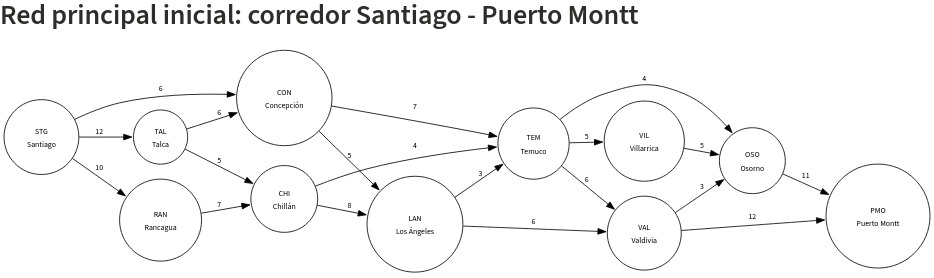
\includegraphics[width=0.92\textwidth]{figuras/fig1_1_red_inicial.png}
  \caption{Red inicial de distribución con las capacidades sobre cada arco.}
  \label{fig:red_inicial}
\end{figure}

\subsection{Grados de los vértices}

$\deg^+(v)$ es el número de arcos que salen de $v$ y $\deg^-(v)$ el número de arcos que entran:

\begin{table}[H]
  \centering
  \small
  \begin{tabular}{lcccccccccccc}
    \toprule
    $v$ & STG & RAN & TAL & CHI & CON & LAN & TEM & VIL & VAL & OSO & PMO & \textbf{Suma} \\
    \midrule
    $\deg^+(v)$ & 3 & 1 & 2 & 2 & 2 & 2 & 3 & 1 & 2 & 1 & 0 & 19 \\
    $\deg^-(v)$ & 0 & 1 & 1 & 2 & 2 & 2 & 3 & 1 & 2 & 3 & 2 & 19 \\
    \textbf{Total} & 3 & 2 & 3 & 4 & 4 & 4 & 6 & 2 & 4 & 4 & 2 & 38 \\
    \bottomrule
  \end{tabular}
  \caption{Grados de salida y entrada de los vértices.}
  \label{tab:grados}
\end{table}

Comprobación: $\sum_{v \in V} \deg^+(v) = \sum_{v \in V} \deg^-(v) = \lvert E\rvert = 19$, porque cada arco aporta una salida y una entrada. El origen no tiene arcos de entrada ($\deg^-(\text{STG}) = 0$) y el destino no tiene arcos de salida ($\deg^+(\text{PMO}) = 0$). Temuco es el centro de mayor grado (6): recibe tres rutas y despacha tres.

\subsection{Auditoría de las restricciones del enunciado}

\begin{table}[H]
  \centering
  \begin{tabular}{p{4.6cm}p{7.4cm}c}
    \toprule
    \textbf{Restricción} & \textbf{Verificación} & \textbf{Cumple} \\
    \midrule
    $10 \le \lvert V\rvert \le 12$ & $\lvert V\rvert = 11$ & Sí \\
    $15 \le \lvert E\rvert \le 20$ & $\lvert E\rvert = 19$ & Sí \\
    $c: E \to \{1,\dots,12\}$ & Las 19 capacidades son enteras y están entre 3 y 12 & Sí \\
    Sin lazos & Ningún arco tiene la forma $(u,u)$ & Sí \\
    Sin arcos repetidos & Los 19 pares ordenados $(u,v)$ son distintos & Sí \\
    Sin arcos recíprocos & Para ningún $(u,v) \in E$ existe $(v,u) \in E$ (red acíclica) & Sí \\
    Ningún vértice aislado & $\deg^+(v) + \deg^-(v) \ge 2$ para todo $v \in V$ (Tabla~\ref{tab:grados}) & Sí \\
    $s \ne t$ & $s = \text{STG}$, $t = \text{PMO}$ & Sí \\
    Al menos dos caminos de $s$ a $t$ & $P_1$ y $P_2$ detallados abajo & Sí \\
    \bottomrule
  \end{tabular}
  \caption{Auditoría de las restricciones del enunciado sobre la red inicial.}
  \label{tab:auditoria}
\end{table}

Dos caminos dirigidos de $s$ a $t$:
\begin{itemize}
  \item $P_1$: $\text{STG} \to \text{CON} \to \text{LAN} \to \text{VAL} \to \text{PMO}$
  \item $P_2$: $\text{STG} \to \text{RAN} \to \text{CHI} \to \text{TEM} \to \text{OSO} \to \text{PMO}$
\end{itemize}

$P_1$ y $P_2$ no comparten ningún arco ni ningún vértice intermedio, de modo que son distintos bajo cualquier lectura de ``caminos distintos''. La aplicación comprueba estas mismas restricciones con código (\texttt{validar\_red} en \texttt{core/validacion.py}): para \texttt{data/initial\_network.json} no reporta ningún error.

\subsection{Interpretación}

\begin{itemize}
  \item \textbf{Sentido único.} Todas las rutas avanzan de norte a sur. Un paquete nunca retrocede, y por eso la red no tiene ciclos ni arcos recíprocos.
  \item \textbf{Rutas alternativas.} Entre Santiago y Puerto Montt hay muchos caminos. Si una ruta se interrumpe, los paquetes pueden desviarse por otros centros; cuánto se pierde depende de las capacidades de las rutas que quedan (sección~4).
  \item \textbf{Cotas inmediatas.} De Santiago pueden salir a lo más $10 + 12 + 6 = 28$ paquetes por hora, y a Puerto Montt pueden entrar a lo más $12 + 11 = 23$. Por lo tanto ningún flujo puede superar 23. El valor exacto depende de las capacidades intermedias, y se calcula mediante el algoritmo de la sección~2.
\end{itemize}

% ==============================================================================
% SECCIÓN 2: INVESTIGACIÓN Y SELECCIÓN DEL ALGORITMO (Rodrigo Pedraza - R9)
% ==============================================================================
\section{Investigación y selección del algoritmo}

\poragregar{Rodrigo Pedraza (Tarea R9)}{%
  Completar a partir de \texttt{docs/fase2-algoritmo.md}:
  \begin{itemize}
    \item Definición de flujo factible, red residual $G_x$, $c_x(u,v)$ y camino aumentante.
    \item Descripción de al menos dos algoritmos alternativos (ej. Ford--Fulkerson, Edmonds--Karp, Dinic).
    \item Tabla comparativa de complejidad temporal, ventajas y desventajas.
    \item Justificación de la elección de Edmonds--Karp y citas bibliográficas confirmadas.
  \end{itemize}
}

% ==============================================================================
% SECCIÓN 3: CORTE MÍNIMO E IMPLEMENTACIÓN (Rodrigo Pedraza - R10)
% ==============================================================================
\section{Teorema de flujo máximo--corte mínimo e implementación}

\poragregar{Rodrigo Pedraza (Tarea R10)}{%
  Explicar el teorema de flujo máximo--corte mínimo ($\lvert x^*\rvert = c(S,T)$), el procedimiento de alcanzabilidad en $G_{x^*}$ desde $s$ para obtener $(S,T)$, y documentar las funciones implementadas en \texttt{core/} (\texttt{flujo\_maximo.py}, \texttt{corte\_minimo.py}, \texttt{resolvedor.py}, \texttt{ediciones.py}, \texttt{validacion.py}).
}

% ==============================================================================
% SECCIÓN 4: RESULTADOS Y ANÁLISIS (Sebastián Pereda - S13)
% ==============================================================================
\section{Resultados y análisis de configuraciones}

\subsection{Configuración 1: Red inicial}
Se ejecutó \texttt{resolver} sobre \texttt{data/initial\_network.json}, con origen STG y destino PMO. El flujo máximo es de $20$ paquetes/hora, obtenido en nueve aumentos. La partición calculada es
\begin{align*}
S_0 &= \{\text{STG},\text{RAN},\text{TAL},\text{CHI},\text{CON},\text{LAN}\},\\
T_0 &= \{\text{TEM},\text{VIL},\text{VAL},\text{OSO},\text{PMO}\}.
\end{align*}
Los arcos del corte son CHI--TEM, CON--TEM, LAN--TEM y LAN--VAL. Sus capacidades suman $4+7+3+6=20$ y todos están saturados. Por tanto, $\lvert x^*\rvert=c(S_0,T_0)=20$. El límite está en las rutas que conectan la zona del Biobío con Temuco y Valdivia, aunque Santiago puede despachar hasta $28$ y Puerto Montt recibir hasta $23$ paquetes/hora.

\begin{figure}[H]
  \centering
  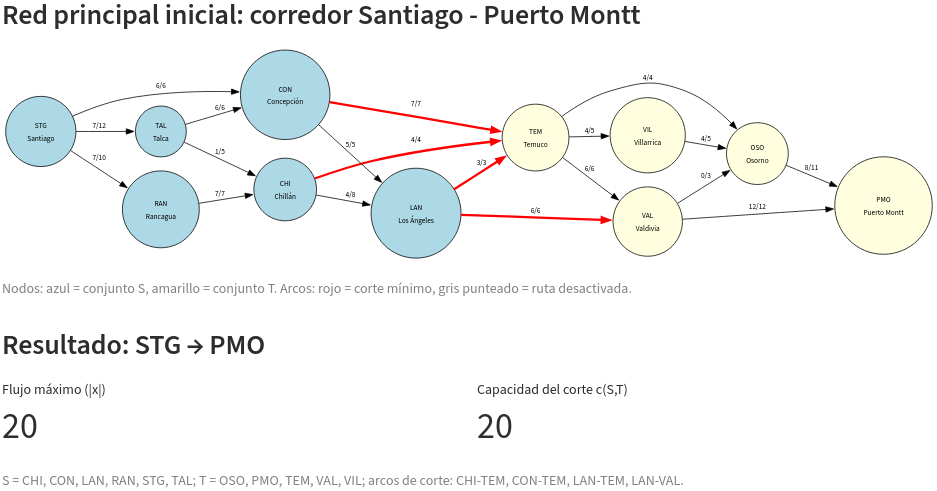
\includegraphics[width=0.95\textwidth]{figuras/fig4_1_red_inicial.png}
  \caption{Resultado del flujo máximo y corte mínimo para la red inicial.}
  \label{fig:res_red_inicial}
\end{figure}

\subsection{Configuración 2: Modificación 1}
En \texttt{data/mod1.json} se desactiva CON--TEM, conservando su capacidad registrada en $7$. La ruta deja de participar en el cálculo y aparece discontinua en la interfaz. El flujo máximo baja a $13$ paquetes/hora, en cinco aumentos. Se mantienen $S=S_0$ y $T=T_0$, pero el corte pierde CON--TEM:
\[
c(S,T)=c(\text{CHI},\text{TEM})+c(\text{LAN},\text{TEM})+
c(\text{LAN},\text{VAL})=4+3+6=13.
\]
Las tres rutas restantes del corte están saturadas. El cierre reduce el transporte en $7$ paquetes/hora, un $35\%$ respecto a la red inicial. Las rutas alternativas no compensan la pérdida porque atraviesan el mismo cuello de botella.

\begin{figure}[H]
  \centering
  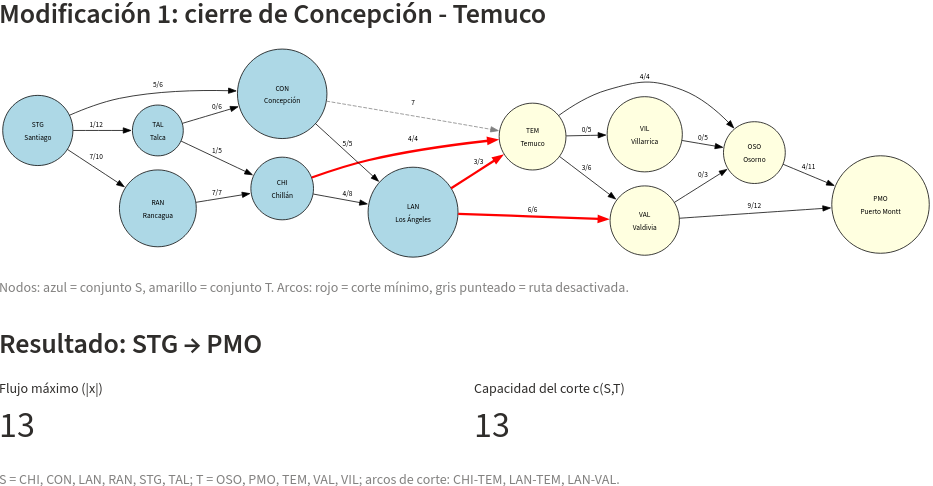
\includegraphics[width=0.95\textwidth]{figuras/fig4_2_mod1.png}
  \caption{Resultado del flujo máximo y corte mínimo para la Modificación 1.}
  \label{fig:res_mod1}
\end{figure}

\subsection{Configuración 3: Modificación 2}
En \texttt{data/mod2.json}, partiendo nuevamente de la red inicial, se amplía CON--TEM de $7$ a $9$ y se agrega CON--VAL con capacidad $8$. El flujo máximo alcanza $23$ paquetes/hora en nueve aumentos: una mejora de $3$ paquetes/hora ($15\%$). Ahora $S=V\setminus\{\text{PMO}\}$ y $T=\{\text{PMO}\}$. El corte se desplaza a las entradas al destino:
\[
c(S,T)=c(\text{VAL},\text{PMO})+c(\text{OSO},\text{PMO})=12+11=23.
\]
Ambas entradas están saturadas. Aumentar otras rutas sin ampliar este acceso final no permite superar $23$. La nueva conexión CON--VAL ya alcanza ese valor por sí sola (prueba S8); la ampliación adicional de CON--TEM no aumenta el máximo de esta configuración. En el flujo obtenido, CON--TEM transporta $4$ de sus $9$ unidades disponibles.

\begin{figure}[H]
  \centering
  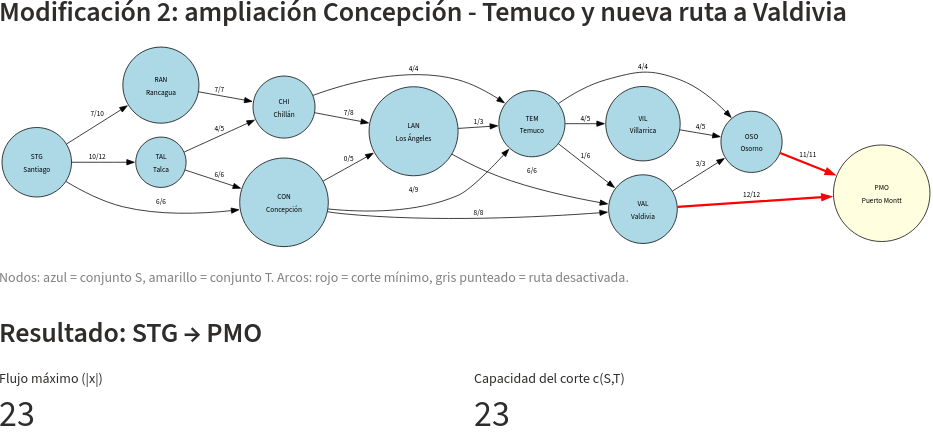
\includegraphics[width=0.95\textwidth]{figuras/fig4_3_mod2.png}
  \caption{Resultado del flujo máximo y corte mínimo para la Modificación 2.}
  \label{fig:res_mod2}
\end{figure}

\subsection{Comparación global}
Las tres configuraciones utilizan los mismos once centros y los terminales STG y PMO. Las modificaciones cubren desactivar, cambiar capacidad y agregar una ruta, sin lazos, arcos repetidos ni recíprocos. \texttt{validar\_red} devuelve una lista vacía para cada archivo.
\begin{table}[H]
  \centering
  \small
  \begin{tabular}{lcc>{\raggedright\arraybackslash}p{4.1cm}>{\raggedright\arraybackslash}p{4.0cm}}
    \toprule
    Red & $\lvert x^*\rvert$ & $c(S,T)$ & Partición & Arcos del corte \\
    \midrule
    Inicial & 20 & 20 & $S_0$, $T_0$ & CHI--TEM, CON--TEM, LAN--TEM, LAN--VAL \\
    Modificación 1 & 13 & 13 & $S_0$, $T_0$ & CHI--TEM, LAN--TEM, LAN--VAL \\
    Modificación 2 & 23 & 23 & $V\setminus\{\text{PMO}\}$, $\{\text{PMO}\}$ & VAL--PMO, OSO--PMO \\
    \bottomrule
  \end{tabular}
  \caption{Comparación de configuraciones; valores en paquetes/hora. Los conjuntos $S_0$ y $T_0$ se definieron en la configuración inicial.}
  \label{tab:comparacion}
\end{table}
Las figuras~\ref{fig:res_red_inicial}--\ref{fig:res_mod2} muestran los resultados de la aplicación. Las tablas de la sección siguiente permiten comprobar capacidad y conservación para cada escenario.

% ==============================================================================
% SECCIÓN 5: VERIFICACIÓN (Sebastián Pereda - S13)
% ==============================================================================
\section{Verificación y caso manual}

\subsection{Resolución manual y redes residuales}
Se resolvió \texttt{data/manual\_case.json}, con seis vértices, ocho arcos, origen $s$ y destino $t$. Se parte de flujo cero y se aplica Edmonds--Karp con BFS y vecinos en orden alfabético. En cada aumento se resta $\delta$ al residual directo y se suma al inverso. Los números de los dibujos siguientes representan capacidades residuales, no las etiquetas $x/c$ de la interfaz.

\begin{table}[H]
  \centering
  \small
  \begin{tabular}{cllcc}
    \toprule
    Aumento & Camino & Residuales antes de aumentar & $\delta$ & $\lvert x\rvert$ \\
    \midrule
    1 & $s\to b\to a\to t$ & $5,6,3$ & 3 & 3 \\
    2 & $s\to b\to d\to t$ & $2,6,9$ & 2 & 5 \\
    3 & $s\to c\to a\to b\to d\to t$ & $7,5,3,4,7$ & 3 & 8 \\
    \bottomrule
  \end{tabular}
  \caption{Registro manual, coincidente con \texttt{iterations} del programa.}
  \label{tab:manual_iteraciones}
\end{table}
El tercer camino recorre $a\to b$, inverso residual del arco original $(b,a)$: cancela sus tres unidades de flujo. Así, $a$ pasa a recibirlas desde $c$ y $b$ redirige las suyas hacia $d$. No se agrega una ruta física recíproca.

\clearpage
\begin{figure}[H]
  \centering
  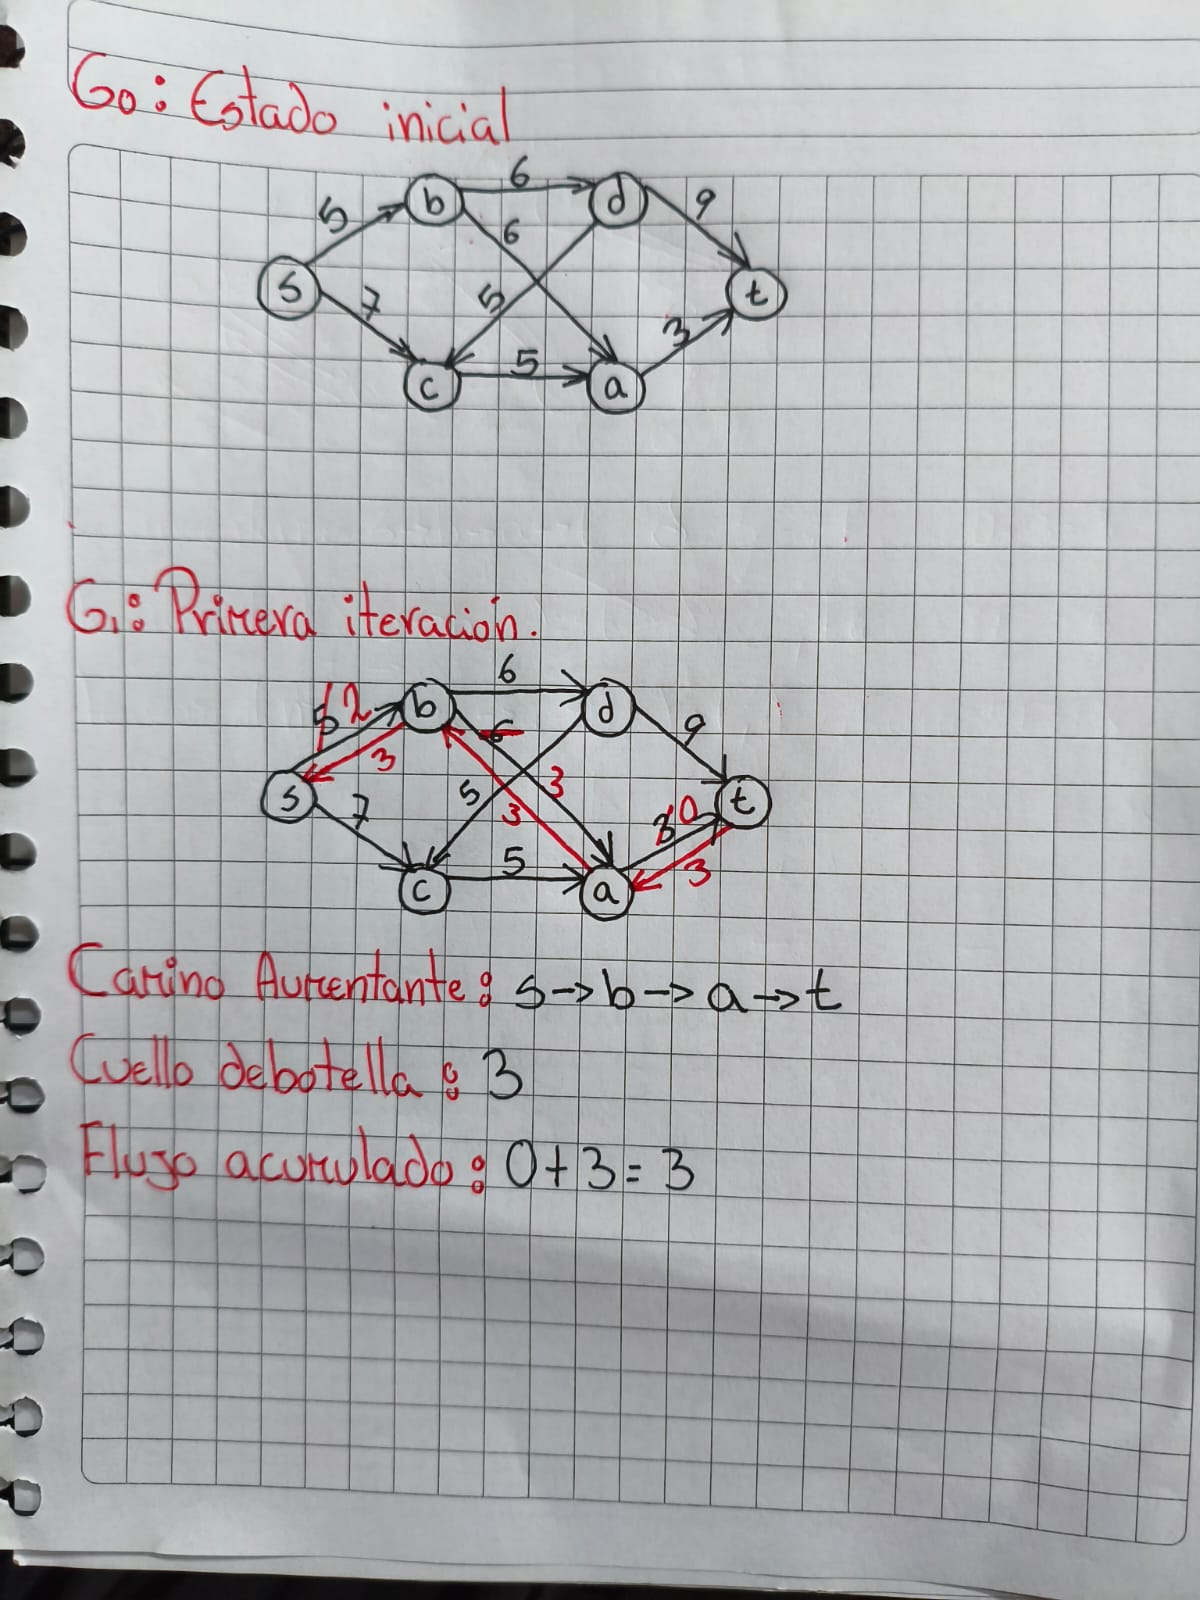
\includegraphics[width=0.93\textwidth,height=0.85\textheight,keepaspectratio]{figuras/manual_01_inicio.png}
  \caption{Cálculo manuscrito de Sebastián: estado inicial y residual tras el primer aumento ($\delta=3$, $\lvert x\rvert=3$).}
  \label{fig:manual_inicio}
\end{figure}

\clearpage
\begin{figure}[H]
  \centering
  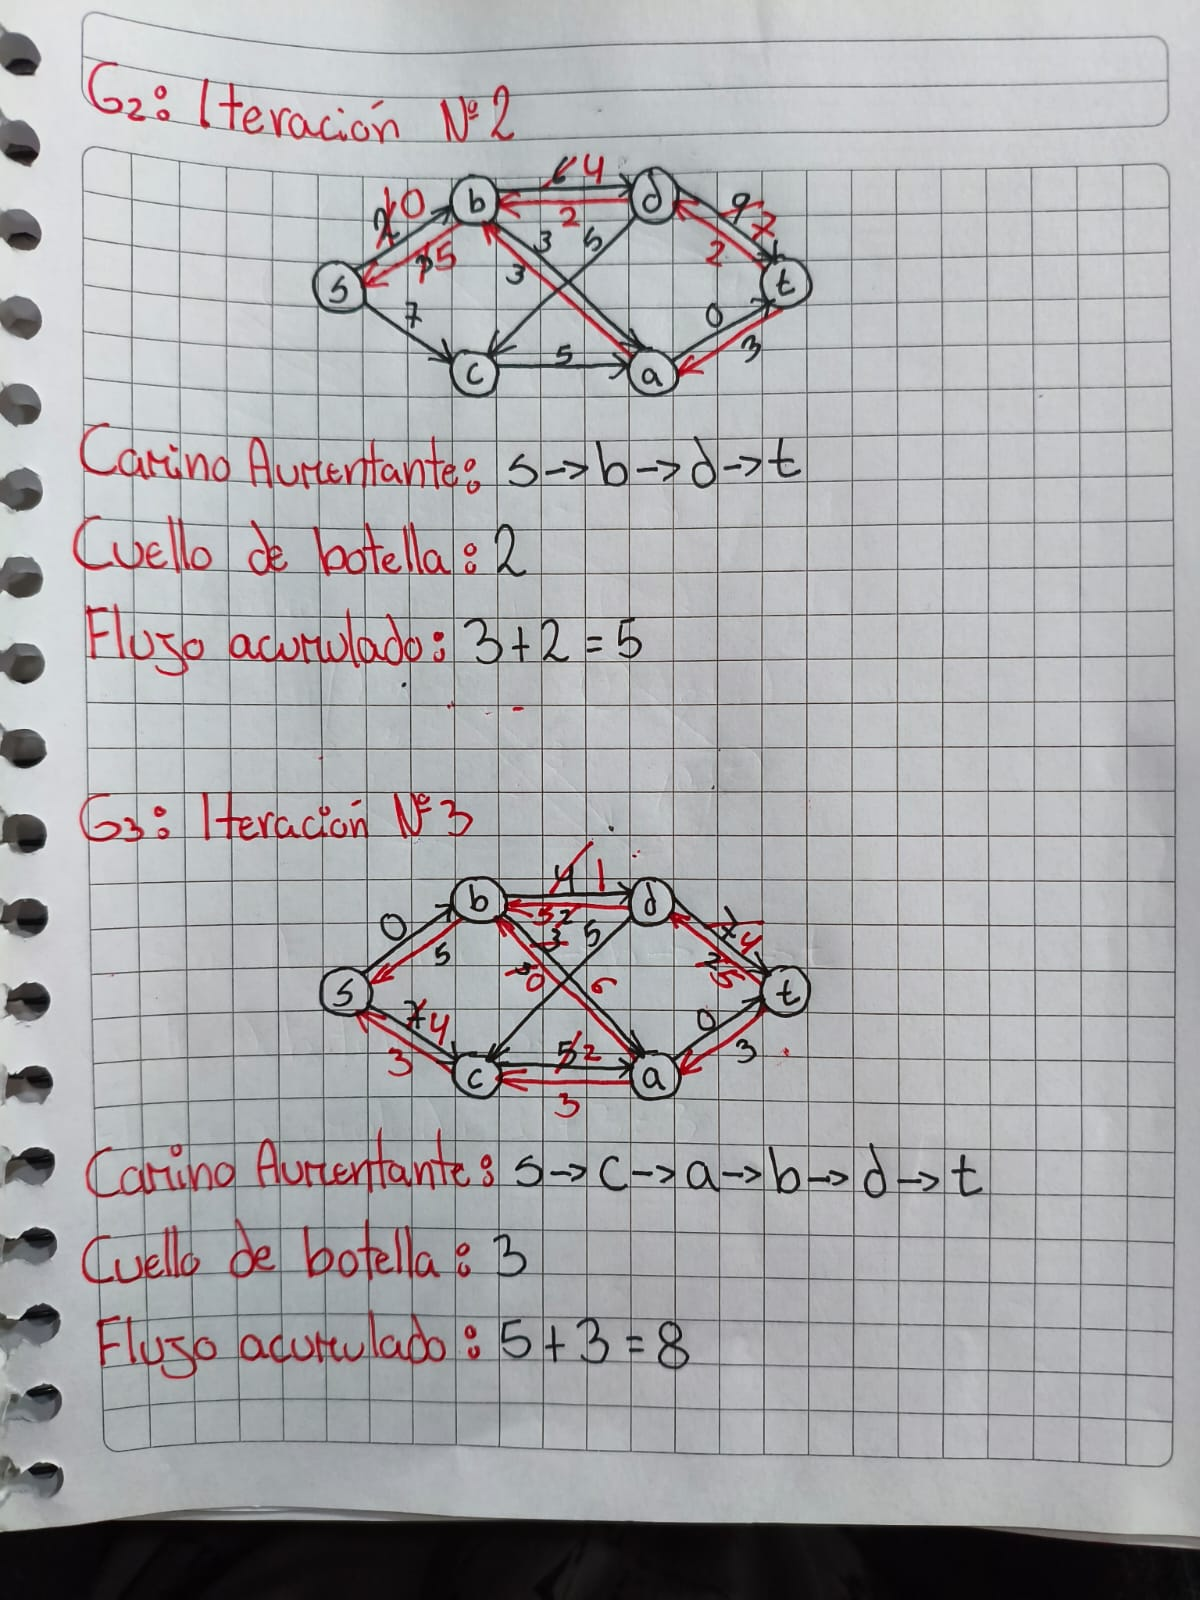
\includegraphics[width=0.93\textwidth,height=0.85\textheight,keepaspectratio]{figuras/manual_02_aumentos.png}
  \caption{Residuales tras los aumentos segundo y tercero. El flujo acumulado pasa de $5$ a $8$ mediante la cancelación por $a\to b$.}
  \label{fig:manual_aumentos}
\end{figure}

\clearpage
\subsection{Parada y certificación de optimalidad}
\begin{figure}[H]
  \centering
  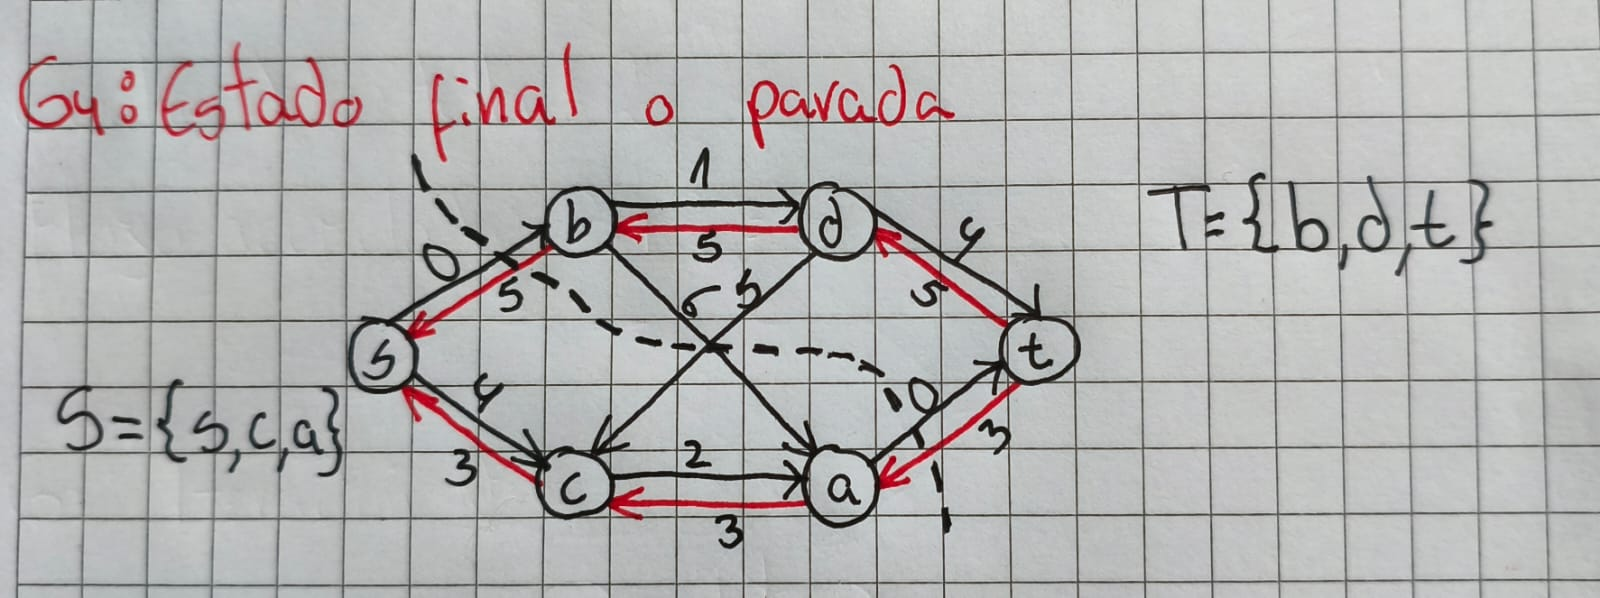
\includegraphics[width=0.98\textwidth]{figuras/manual_03_corte.png}
  \caption{Residual final y separación de $S=\{s,a,c\}$ y $T=\{b,d,t\}$. El estado $G_4$ del manuscrito es la búsqueda de parada; hubo tres aumentos.}
  \label{fig:manual_corte}
\end{figure}

\textbf{Justificación:} Al intentar nuevamente un camino aumentante desde el origen $s$, solo se logra avanzar hasta el nodo $a$ (pasando por $c$), donde nos encontramos bloqueados para seguir hacia el destino $t$: el arco directo $(a,t)$ ya tiene su máxima capacidad utilizada ($c_x(a,t)=0$) y el arco inverso $(a,b)$ también quedó en $0$ al cancelarse el flujo previo de $(b,a)$ en la iteración 3. Por lo tanto, el conjunto alcanzable $S=\{s,a,c\}$ queda aislado del resto de la red ($T=\{b,d,t\}$) y ahí se cierra el flujo.

Aquí \emph{aislado} significa que no hay arcos de capacidad residual positiva que permitan salir de $S$ hacia $T$; sí existen conexiones en la red original y arcos residuales en sentido contrario.

\textbf{Certificación de optimalidad:} Los únicos arcos originales que cruzan de $S$ hacia $T$ son $(s,b)$ y $(a,t)$, ambos saturados, con capacidad total $c(S,T)=5+3=8$ paquetes/hora. Como todo flujo factible cumple $\lvert x\rvert\le c(S,T)$ y aquí se obtiene $\lvert x\rvert=c(S,T)=8$, se certifica que el flujo es \textbf{máximo} y el corte $(S,T)$ es \textbf{mínimo}.

\subsection{Flujo final y contraste con el programa}
El flujo final se recupera de cada arco original como $x(u,v)=c(u,v)-c_x(u,v)$. La tabla~\ref{tab:manual_capacidad} muestra que todos los valores son enteros y satisfacen $0\le x(u,v)\le c(u,v)$.
\begin{table}[H]
  \centering
  \begin{tabular}{lrrrr}
    \toprule
    Arco & $c$ & $x$ manual & $x$ programa & $c_x$ directo final \\
    \midrule
    $(s,b)$ & 5 & 5 & 5 & 0 \\
    $(s,c)$ & 7 & 3 & 3 & 4 \\
    $(b,a)$ & 6 & 0 & 0 & 6 \\
    $(b,d)$ & 6 & 5 & 5 & 1 \\
    $(c,a)$ & 5 & 3 & 3 & 2 \\
    $(d,c)$ & 5 & 0 & 0 & 5 \\
    $(a,t)$ & 3 & 3 & 3 & 0 \\
    $(d,t)$ & 9 & 5 & 5 & 4 \\
    \bottomrule
  \end{tabular}
  \caption{Capacidad y flujo final por arco del caso manual, contrastados con \texttt{flows}.}
  \label{tab:manual_capacidad}
\end{table}

\begin{table}[H]
  \centering
  \begin{tabular}{lrrr}
    \toprule
    Nodo & Entrada & Salida & Entrada menos salida \\
    \midrule
    $a$ & 3 & 3 & 0 \\
    $b$ & 5 & 5 & 0 \\
    $c$ & 3 & 3 & 0 \\
    $d$ & 5 & 5 & 0 \\
    \bottomrule
  \end{tabular}
  \caption{Conservación en los nodos intermedios del caso manual, coincidente con \texttt{conservation\_table}.}
  \label{tab:manual_conservacion}
\end{table}
El origen entrega $5+3=8$ y el destino recibe $3+5=8$ paquetes/hora. La salida de \texttt{resolver} coincide con el cálculo manual en los tres caminos, los cuellos de botella $(3,2,3)$, los flujos por arco y la partición del corte. La búsqueda final sin camino no agrega una fila a \texttt{iterations}. No se observaron diferencias entre ambas resoluciones.

\begin{figure}[H]
  \centering
  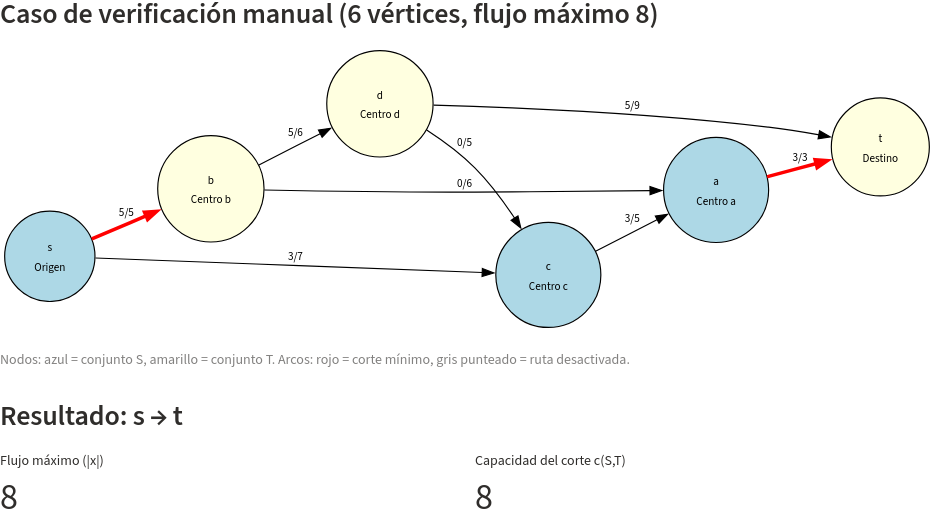
\includegraphics[width=0.95\textwidth]{figuras/fig5_1_caso_manual.png}
  \caption{Resultado del flujo máximo y corte mínimo para el caso de verificación manual.}
  \label{fig:res_caso_manual}
\end{figure}

\subsection{Comprobaciones de las tres configuraciones}
Las siguientes tablas se obtuvieron de \texttt{flows}, las capacidades de los JSON y \texttt{checks} al ejecutar \texttt{resolver} para cada configuración. \texttt{core/verificacion.py} recalcula las comprobaciones desde la red y los flujos, sin consultar el motor ni su residual.

\begin{table}[H]
  \centering
  \small
  \begin{tabular}{lccc}
    \toprule
    Arco & Inicial: $x/c$ & Modificación 1: $x/c$ & Modificación 2: $x/c$ \\
    \midrule
    STG--RAN & 7/10 & 7/10 & 7/10 \\
    STG--TAL & 7/12 & 1/12 & 10/12 \\
    STG--CON & 6/6 & 5/6 & 6/6 \\
    RAN--CHI & 7/7 & 7/7 & 7/7 \\
    TAL--CHI & 1/5 & 1/5 & 4/5 \\
    TAL--CON & 6/6 & 0/6 & 6/6 \\
    CHI--LAN & 4/8 & 4/8 & 7/8 \\
    CHI--TEM & 4/4 & 4/4 & 4/4 \\
    CON--LAN & 5/5 & 5/5 & 0/5 \\
    CON--TEM & 7/7 & Inactivo & 4/9 \\
    LAN--TEM & 3/3 & 3/3 & 1/3 \\
    LAN--VAL & 6/6 & 6/6 & 6/6 \\
    TEM--VIL & 4/5 & 0/5 & 4/5 \\
    TEM--VAL & 6/6 & 3/6 & 1/6 \\
    TEM--OSO & 4/4 & 4/4 & 4/4 \\
    VIL--OSO & 4/5 & 0/5 & 4/5 \\
    VAL--OSO & 0/3 & 0/3 & 3/3 \\
    VAL--PMO & 12/12 & 9/12 & 12/12 \\
    OSO--PMO & 8/11 & 4/11 & 11/11 \\
    CON--VAL & No existe & No existe & 8/8 \\
    \bottomrule
  \end{tabular}
  \caption{Verificación de capacidad por arco: en toda ruta activa, $x$ es entero y $0\le x\le c$. Un arco inactivo no aparece en \texttt{flows}.}
  \label{tab:capacidades_configuraciones}
\end{table}

\begin{table}[H]
  \centering
  \small
  \begin{tabular}{lccc}
    \toprule
    Nodo & Inicial: entra/sale & Modificación 1: entra/sale & Modificación 2: entra/sale \\
    \midrule
    CHI & 8/8 & 8/8 & 11/11 \\
    CON & 12/12 & 5/5 & 12/12 \\
    LAN & 9/9 & 9/9 & 7/7 \\
    OSO & 8/8 & 4/4 & 11/11 \\
    RAN & 7/7 & 7/7 & 7/7 \\
    TAL & 7/7 & 1/1 & 10/10 \\
    TEM & 14/14 & 7/7 & 9/9 \\
    VAL & 12/12 & 9/9 & 15/15 \\
    VIL & 4/4 & 0/0 & 4/4 \\
    \bottomrule
  \end{tabular}
  \caption{Conservación por nodo intermedio. Entrada y salida coinciden en todas las filas; STG y PMO se excluyen por ser los terminales.}
  \label{tab:conservacion_configuraciones}
\end{table}

\begin{table}[H]
  \centering
  \small
  \begin{tabular}{lcccc}
    \toprule
    Caso & Capacidad & Conservación & $\lvert x\rvert=c(S,T)$ & Dualidad \\
    \midrule
    Inicial & Cumple & Cumple & $20=20$ & Cumple \\
    Modificación 1 & Cumple & Cumple & $13=13$ & Cumple \\
    Modificación 2 & Cumple & Cumple & $23=23$ & Cumple \\
    Manual & Cumple & Cumple & $8=8$ & Cumple \\
    \bottomrule
  \end{tabular}
  \caption{Resumen de \texttt{checks}. Dualidad exige además $s\in S$ y $t\notin S$.}
  \label{tab:checks}
\end{table}

\subsection{Pruebas automáticas}
Las pruebas S7--S11 comprueban resultados conocidos, modificaciones, casos borde y errores de validación. Como contraste independiente, \texttt{brute\_force\_min\_cut} enumera todos los cortes de las tres redes de referencia y de veinte redes aleatorias válidas de seis nodos (semilla 1), y compara el mínimo con el flujo calculado. La suite se ejecuta desde la raíz con \texttt{python -m unittest}. Estas pruebas complementan el cálculo manual; la revisión interactiva de la interfaz corresponde a S14.

% ==============================================================================
% SECCIÓN 6: REFERENCIAS (Rodrigo Pedraza - R11)
% ==============================================================================
\section{Referencias}

\poragregar{Rodrigo Pedraza (Tarea R11)}{%
  Agregar referencias académicas y técnicas verificadas (ej. Cormen et al. CLRS, Kleinberg \& Tardos, documentación de Python/Streamlit/Graphviz) usando \texttt{\textbackslash begin\{thebibliography\}} o BibLaTeX.
}

\end{document}
